\Author{\daAuthorTwo}

\subsubsection{Dart}
Dart is a programming language initially designed for web development, with the goal, of replacing JavaScript, in mind. Today it gets used in a variety of software products, mainly because of the flutter framework. It can be compiled for many platforms and architectures (ARM, x64, RISC-V, JavaScript or WebAssembly) and is loved for its combination of High-Level Features, with practical language features like Garbage collection and optional Type annotation. It was developed by Google and is now an open-source project.

\blankLine

\autocite{BibEntry}

\begin{figure}
    \center
    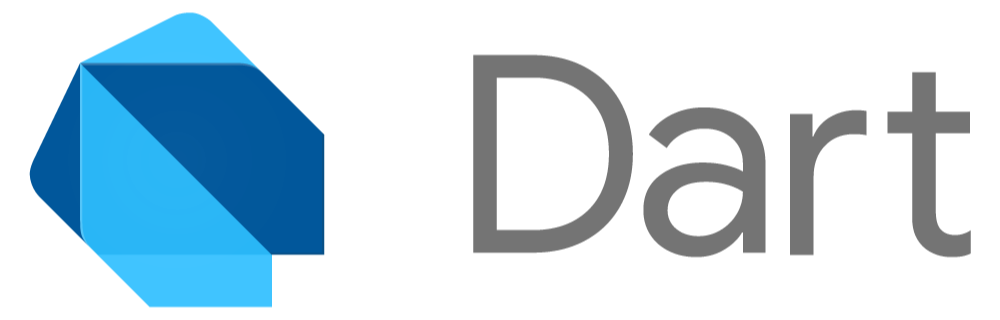
\includegraphics [width=0.6\textwidth] {images/Technologies/dartLogo.png}
    \caption{Dart Logo Source}
\end{figure}

\subsubsection{Flutter}
Flutter is an Open-Source software development framework. It allows programmers to compile their application for different platforms including Web, macOS, IOS as well as Windows and any type of Linux-based systems, all from one code-base, written in Dart. This allows for more efficient and faster cross-platform development. Another benefit of Google's toolkit are the highly customizable predefined UI components. Developers can mix and match these components however needed which makes them an applicable choice.

\blankLine

We chose flutter mainly for these reasons, but also because of our previous experience with Java to which Dart is quite similar. Through it, we were able to get started quickly, learn what we need along the way. Having a design through the components was also very helpful and saved us some time. 

\blankLine

\autocite{flutterReadMe}
\autocite{dagne2019flutter}

\blankLine


\includegraphics [width=0.6\textwidth] {images/Technologies/flutterLogo.png}
\newpage